\documentclass[twoside]{book}

% Packages required by doxygen
\usepackage{fixltx2e}
\usepackage{calc}
\usepackage{doxygen}
\usepackage{graphicx}
\usepackage[utf8]{inputenc}
\usepackage{makeidx}
\usepackage{multicol}
\usepackage{multirow}
\PassOptionsToPackage{warn}{textcomp}
\usepackage{textcomp}
\usepackage[nointegrals]{wasysym}
\usepackage[table]{xcolor}

% Font selection
\usepackage[T1]{fontenc}
\usepackage{mathptmx}
\usepackage[scaled=.90]{helvet}
\usepackage{courier}
\usepackage{amssymb}
\usepackage{sectsty}
\renewcommand{\familydefault}{\sfdefault}
\allsectionsfont{%
  \fontseries{bc}\selectfont%
  \color{darkgray}%
}
\renewcommand{\DoxyLabelFont}{%
  \fontseries{bc}\selectfont%
  \color{darkgray}%
}
\newcommand{\+}{\discretionary{\mbox{\scriptsize$\hookleftarrow$}}{}{}}

% Page & text layout
\usepackage{geometry}
\geometry{%
  a4paper,%
  top=2.5cm,%
  bottom=2.5cm,%
  left=2.5cm,%
  right=2.5cm%
}
\tolerance=750
\hfuzz=15pt
\hbadness=750
\setlength{\emergencystretch}{15pt}
\setlength{\parindent}{0cm}
\setlength{\parskip}{0.2cm}
\makeatletter
\renewcommand{\paragraph}{%
  \@startsection{paragraph}{4}{0ex}{-1.0ex}{1.0ex}{%
    \normalfont\normalsize\bfseries\SS@parafont%
  }%
}
\renewcommand{\subparagraph}{%
  \@startsection{subparagraph}{5}{0ex}{-1.0ex}{1.0ex}{%
    \normalfont\normalsize\bfseries\SS@subparafont%
  }%
}
\makeatother

% Headers & footers
\usepackage{fancyhdr}
\pagestyle{fancyplain}
\fancyhead[LE]{\fancyplain{}{\bfseries\thepage}}
\fancyhead[CE]{\fancyplain{}{}}
\fancyhead[RE]{\fancyplain{}{\bfseries\leftmark}}
\fancyhead[LO]{\fancyplain{}{\bfseries\rightmark}}
\fancyhead[CO]{\fancyplain{}{}}
\fancyhead[RO]{\fancyplain{}{\bfseries\thepage}}
\fancyfoot[LE]{\fancyplain{}{}}
\fancyfoot[CE]{\fancyplain{}{}}
\fancyfoot[RE]{\fancyplain{}{\bfseries\scriptsize Generated on Sat Dec 30 2017 01\+:40\+:26 for My Project by Doxygen }}
\fancyfoot[LO]{\fancyplain{}{\bfseries\scriptsize Generated on Sat Dec 30 2017 01\+:40\+:26 for My Project by Doxygen }}
\fancyfoot[CO]{\fancyplain{}{}}
\fancyfoot[RO]{\fancyplain{}{}}
\renewcommand{\footrulewidth}{0.4pt}
\renewcommand{\chaptermark}[1]{%
  \markboth{#1}{}%
}
\renewcommand{\sectionmark}[1]{%
  \markright{\thesection\ #1}%
}

% Indices & bibliography
\usepackage{natbib}
\usepackage[titles]{tocloft}
\setcounter{tocdepth}{3}
\setcounter{secnumdepth}{5}
\makeindex

% Hyperlinks (required, but should be loaded last)
\usepackage{ifpdf}
\ifpdf
  \usepackage[pdftex,pagebackref=true]{hyperref}
\else
  \usepackage[ps2pdf,pagebackref=true]{hyperref}
\fi
\hypersetup{%
  colorlinks=true,%
  linkcolor=blue,%
  citecolor=blue,%
  unicode%
}

% Custom commands
\newcommand{\clearemptydoublepage}{%
  \newpage{\pagestyle{empty}\cleardoublepage}%
}


%===== C O N T E N T S =====

\begin{document}

% Titlepage & ToC
\hypersetup{pageanchor=false,
             bookmarks=true,
             bookmarksnumbered=true,
             pdfencoding=unicode
            }
\pagenumbering{roman}
\begin{titlepage}
\vspace*{7cm}
\begin{center}%
{\Large My Project }\\
\vspace*{1cm}
{\large Generated by Doxygen 1.8.8}\\
\vspace*{0.5cm}
{\small Sat Dec 30 2017 01:40:26}\\
\end{center}
\end{titlepage}
\clearemptydoublepage
\tableofcontents
\clearemptydoublepage
\pagenumbering{arabic}
\hypersetup{pageanchor=true}

%--- Begin generated contents ---
\chapter{Data Structure Index}
\section{Data Structures}
Here are the data structures with brief descriptions\+:\begin{DoxyCompactList}
\item\contentsline{section}{\hyperlink{structLwColor}{Lw\+Color} }{\pageref{structLwColor}}{}
\end{DoxyCompactList}

\chapter{File Index}
\section{File List}
Here is a list of all documented files with brief descriptions\+:\begin{DoxyCompactList}
\item\contentsline{section}{\hyperlink{ledCryptoTree_8h}{led\+Crypto\+Tree.\+h} }{\pageref{ledCryptoTree_8h}}{}
\item\contentsline{section}{\hyperlink{ledCryptoTree_8ino}{led\+Crypto\+Tree.\+ino} }{\pageref{ledCryptoTree_8ino}}{}
\end{DoxyCompactList}

\chapter{Data Structure Documentation}
\hypertarget{structLwColor}{\section{Lw\+Color Struct Reference}
\label{structLwColor}\index{Lw\+Color@{Lw\+Color}}
}
\subsection*{Data Fields}
\begin{DoxyCompactItemize}
\item 
byte \hyperlink{structLwColor_a8493c887c20eb410545f83f2c4fb2ced}{red}
\item 
byte \hyperlink{structLwColor_a4da7ab43afe92d21d7f8fcebbee1ff3d}{green}
\item 
byte \hyperlink{structLwColor_a3f00195781bdbfd0db16c94f8ea85427}{blue}
\end{DoxyCompactItemize}


\subsection{Field Documentation}
\hypertarget{structLwColor_a3f00195781bdbfd0db16c94f8ea85427}{\index{Lw\+Color@{Lw\+Color}!blue@{blue}}
\index{blue@{blue}!Lw\+Color@{Lw\+Color}}
\subsubsection[{blue}]{\setlength{\rightskip}{0pt plus 5cm}byte Lw\+Color\+::blue}}\label{structLwColor_a3f00195781bdbfd0db16c94f8ea85427}
The blue byte \hypertarget{structLwColor_a4da7ab43afe92d21d7f8fcebbee1ff3d}{\index{Lw\+Color@{Lw\+Color}!green@{green}}
\index{green@{green}!Lw\+Color@{Lw\+Color}}
\subsubsection[{green}]{\setlength{\rightskip}{0pt plus 5cm}byte Lw\+Color\+::green}}\label{structLwColor_a4da7ab43afe92d21d7f8fcebbee1ff3d}
The green byte \hypertarget{structLwColor_a8493c887c20eb410545f83f2c4fb2ced}{\index{Lw\+Color@{Lw\+Color}!red@{red}}
\index{red@{red}!Lw\+Color@{Lw\+Color}}
\subsubsection[{red}]{\setlength{\rightskip}{0pt plus 5cm}byte Lw\+Color\+::red}}\label{structLwColor_a8493c887c20eb410545f83f2c4fb2ced}
The red byte 

The documentation for this struct was generated from the following file\+:\begin{DoxyCompactItemize}
\item 
\hyperlink{ledCryptoTree_8h}{led\+Crypto\+Tree.\+h}\end{DoxyCompactItemize}

\chapter{File Documentation}
\hypertarget{ledCryptoTree_8h}{\section{led\+Crypto\+Tree.\+h File Reference}
\label{ledCryptoTree_8h}\index{led\+Crypto\+Tree.\+h@{led\+Crypto\+Tree.\+h}}
}
This graph shows which files directly or indirectly include this file\+:
\nopagebreak
\begin{figure}[H]
\begin{center}
\leavevmode
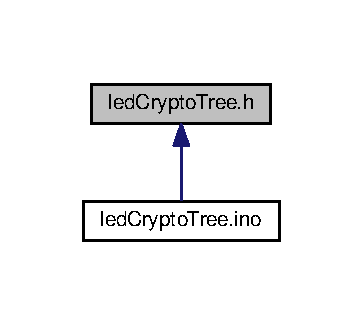
\includegraphics[width=174pt]{ledCryptoTree_8h__dep__incl}
\end{center}
\end{figure}
\subsection*{Data Structures}
\begin{DoxyCompactItemize}
\item 
struct \hyperlink{structLwColor}{Lw\+Color}
\end{DoxyCompactItemize}
\subsection*{Macros}
\begin{DoxyCompactItemize}
\item 
\hypertarget{ledCryptoTree_8h_ac6e010d032716411ea8f8e79ebb7c211}{\#define {\bfseries C\+O\+L\+O\+R\+\_\+\+V\+A\+L\+\_\+\+M\+I\+N}~0}\label{ledCryptoTree_8h_ac6e010d032716411ea8f8e79ebb7c211}

\item 
\hypertarget{ledCryptoTree_8h_ab69ef4bdb41b6ec3a19d667658eb7374}{\#define {\bfseries C\+O\+L\+O\+R\+\_\+\+V\+A\+L\+\_\+\+M\+A\+X}~255}\label{ledCryptoTree_8h_ab69ef4bdb41b6ec3a19d667658eb7374}

\item 
\hypertarget{ledCryptoTree_8h_a264cecc46b0e72ff1d514ab3477e6c14}{\#define {\bfseries S\+E\+R\+I\+A\+L\+\_\+\+D\+A\+T\+A\+\_\+\+R\+A\+T\+E}~9600}\label{ledCryptoTree_8h_a264cecc46b0e72ff1d514ab3477e6c14}

\item 
\hypertarget{ledCryptoTree_8h_a8731de63566896d146d8c1601e72c55f}{\#define {\bfseries N\+E\+O\+P\+I\+X\+\_\+\+T\+Y\+P\+E}~N\+E\+O\+\_\+\+G\+R\+B + N\+E\+O\+\_\+\+K\+H\+Z800}\label{ledCryptoTree_8h_a8731de63566896d146d8c1601e72c55f}

\item 
\hypertarget{ledCryptoTree_8h_a54f23098daac0b52e43a87cffa2e01a5}{\#define {\bfseries S\+E\+R\+I\+A\+L\+\_\+\+I\+N\+T\+R\+O\+\_\+\+T\+E\+X\+T}~\char`\"{}1-\/3 are state chamges 4-\/9 are light shows\char`\"{}}\label{ledCryptoTree_8h_a54f23098daac0b52e43a87cffa2e01a5}

\item 
\hypertarget{ledCryptoTree_8h_a05a34d6e9163d55f88b139aafbe98751}{\#define {\bfseries V\+E\+R\+T\+I\+C\+A\+L\+\_\+\+P\+I\+N}~6}\label{ledCryptoTree_8h_a05a34d6e9163d55f88b139aafbe98751}

\item 
\hypertarget{ledCryptoTree_8h_ae0fa1b3d0708f0077f35fe8d12359fd6}{\#define {\bfseries V\+E\+R\+T\+I\+C\+A\+L\+\_\+\+N\+U\+M}~10}\label{ledCryptoTree_8h_ae0fa1b3d0708f0077f35fe8d12359fd6}

\item 
\hypertarget{ledCryptoTree_8h_ad8c173c9297c85133ed8ed8706bbadc3}{\#define {\bfseries S\+P\+I\+R\+A\+L\+\_\+\+P\+I\+N}~7}\label{ledCryptoTree_8h_ad8c173c9297c85133ed8ed8706bbadc3}

\item 
\hypertarget{ledCryptoTree_8h_aa538a087a83088ce835b5f6c5e2243f4}{\#define {\bfseries S\+P\+I\+R\+A\+L\+\_\+\+N\+U\+M}~10}\label{ledCryptoTree_8h_aa538a087a83088ce835b5f6c5e2243f4}

\item 
\hypertarget{ledCryptoTree_8h_a984f75fadda302389d21d8352734fe71}{\#define {\bfseries F\+A\+I\+R\+Y\+\_\+\+P\+I\+N}~9}\label{ledCryptoTree_8h_a984f75fadda302389d21d8352734fe71}

\item 
\hypertarget{ledCryptoTree_8h_a770d0752fe6fe4f4c8f136225bf7617b}{\#define {\bfseries L\+W\+\_\+\+B\+L\+A\+C\+K}~(\hyperlink{structLwColor}{Lw\+Color})\{0x00, 0x00, 0x00\}}\label{ledCryptoTree_8h_a770d0752fe6fe4f4c8f136225bf7617b}

\item 
\hypertarget{ledCryptoTree_8h_ae519211e5db44cd96cf7490726f1a0fa}{\#define {\bfseries L\+W\+\_\+\+R\+E\+D}~(\hyperlink{structLwColor}{Lw\+Color})\{0xff, 0x00, 0x00\}}\label{ledCryptoTree_8h_ae519211e5db44cd96cf7490726f1a0fa}

\item 
\hypertarget{ledCryptoTree_8h_ae2eac2a871da4f7ac100c5e1f233187e}{\#define {\bfseries L\+W\+\_\+\+G\+R\+E\+E\+N}~(\hyperlink{structLwColor}{Lw\+Color})\{0x00, 0xff, 0x00\}}\label{ledCryptoTree_8h_ae2eac2a871da4f7ac100c5e1f233187e}

\item 
\hypertarget{ledCryptoTree_8h_a000690e93da3628682716fed73c930ae}{\#define {\bfseries L\+W\+\_\+\+B\+L\+U\+E}~(\hyperlink{structLwColor}{Lw\+Color})\{0x00, 0x00, 0xff\}}\label{ledCryptoTree_8h_a000690e93da3628682716fed73c930ae}

\item 
\hypertarget{ledCryptoTree_8h_ada03acd162e17f37e9d53c71caa431ac}{\#define {\bfseries L\+W\+\_\+\+W\+H\+I\+T\+E}~(\hyperlink{structLwColor}{Lw\+Color})\{0xff, 0xff, 0xff\}}\label{ledCryptoTree_8h_ada03acd162e17f37e9d53c71caa431ac}

\item 
\hypertarget{ledCryptoTree_8h_ac4323b7442ac82e58d8bdcfffe8f3b60}{\#define {\bfseries C\+O\+L\+O\+R\+\_\+\+S\+I\+N\+\_\+\+F\+U\+L\+L}(f, i, c)~(((sin(f + i) $\ast$ 127 + 128) / C\+O\+L\+O\+R\+\_\+\+V\+A\+L\+\_\+\+M\+A\+X) $\ast$ c)}\label{ledCryptoTree_8h_ac4323b7442ac82e58d8bdcfffe8f3b60}

\item 
\hypertarget{ledCryptoTree_8h_a17d796da9ba678980b1b5c7fe649cc1f}{\#define {\bfseries R\+G\+B\+\_\+\+S\+I\+N\+E}(f, i)~(sin(f + i) $\ast$ 127 + 128)}\label{ledCryptoTree_8h_a17d796da9ba678980b1b5c7fe649cc1f}

\item 
\hypertarget{ledCryptoTree_8h_a30574ececd9f3b347d06ba0a77bb3e6a}{\#define {\bfseries C\+O\+L\+O\+R\+\_\+\+S\+I\+N}(p, c)~((R\+G\+B\+\_\+\+S\+I\+N\+E(p, 0) / C\+O\+L\+O\+R\+\_\+\+V\+A\+L\+\_\+\+M\+A\+X) $\ast$ c)}\label{ledCryptoTree_8h_a30574ececd9f3b347d06ba0a77bb3e6a}

\item 
\hypertarget{ledCryptoTree_8h_a600959bd1d21f9b4700c431d37027921}{\#define {\bfseries D\+I\+V\+\_\+\+C\+O\+N\+V}(a, b)~((byte)(a / b))}\label{ledCryptoTree_8h_a600959bd1d21f9b4700c431d37027921}

\item 
\hypertarget{ledCryptoTree_8h_abd9d3d96840e6c9a53e9e2973173abad}{\#define {\bfseries C\+O\+L\+O\+R\+\_\+\+S\+I\+N\+\_\+\+C\+O\+N\+V}(p, c)~((byte)C\+O\+L\+O\+R\+\_\+\+S\+I\+N(p, c))}\label{ledCryptoTree_8h_abd9d3d96840e6c9a53e9e2973173abad}

\item 
\hypertarget{ledCryptoTree_8h_a1ca27dc55f840013cd6bc3387f6a500a}{\#define {\bfseries C\+O\+L\+O\+R\+\_\+\+V\+A\+L\+\_\+\+R\+A\+N\+D}~((byte)random(C\+O\+L\+O\+R\+\_\+\+V\+A\+L\+\_\+\+M\+I\+N, C\+O\+L\+O\+R\+\_\+\+V\+A\+L\+\_\+\+M\+A\+X))}\label{ledCryptoTree_8h_a1ca27dc55f840013cd6bc3387f6a500a}

\end{DoxyCompactItemize}
\subsection*{Typedefs}
\begin{DoxyCompactItemize}
\item 
\hypertarget{ledCryptoTree_8h_a153ccb39776befaf95652c44d0f12c97}{typedef uint16\+\_\+t {\bfseries Pixel}}\label{ledCryptoTree_8h_a153ccb39776befaf95652c44d0f12c97}

\item 
\hypertarget{ledCryptoTree_8h_af635e7662397c0219198ece6cfc31b81}{typedef Adafruit\+\_\+\+Neo\+Pixel {\bfseries Neo\+Pix}}\label{ledCryptoTree_8h_af635e7662397c0219198ece6cfc31b81}

\item 
typedef enum \hyperlink{ledCryptoTree_8h_ab3047c9bf4528fcc2e0f4360115b9f79}{Goals} \hyperlink{ledCryptoTree_8h_a0ba78d87f754b7f0ab05e1534dfb54f4}{Goals}
\item 
\hypertarget{ledCryptoTree_8h_aedcf872dd88af5625a8c0b7d5927dc78}{typedef struct \hyperlink{structLwColor}{Lw\+Color} {\bfseries Lw\+Color}}\label{ledCryptoTree_8h_aedcf872dd88af5625a8c0b7d5927dc78}

\end{DoxyCompactItemize}
\subsection*{Enumerations}
\begin{DoxyCompactItemize}
\item 
enum \hyperlink{ledCryptoTree_8h_ab3047c9bf4528fcc2e0f4360115b9f79}{Goals} \{ {\bfseries N\+O\+N\+E} = 0, 
{\bfseries S\+M\+A\+L\+L} = 1, 
{\bfseries M\+E\+D\+I\+U\+M} = 2, 
{\bfseries B\+I\+G} = 4
 \}
\end{DoxyCompactItemize}
\subsection*{Functions}
\begin{DoxyCompactItemize}
\item 
void \hyperlink{ledCryptoTree_8h_ad4e0c88560cf11558cafaded5334a413}{setup\+Serial} ()
\item 
void \hyperlink{ledCryptoTree_8h_a3d4a7770febd94a46810f36c3d2ac32e}{setup\+Neopix} ()
\item 
void \hyperlink{ledCryptoTree_8h_a2fb2eb2b13bc6122f9c89d000e2d7d01}{parse\+Serial} ()
\item 
void \hyperlink{ledCryptoTree_8h_a9e090d395c12709aa3a4ff2754b30828}{parse\+Goals} ()
\item 
void \hyperlink{ledCryptoTree_8h_abc190235cc82d8ca7c65eb0b30dfe689}{simple\+Fade\+In} (int, int)
\item 
void \hyperlink{ledCryptoTree_8h_ac397f7275df5de9f78ead96caa7699d1}{simple\+Fade\+Out} (int, int)
\item 
void \hyperlink{ledCryptoTree_8h_a8aa6221c69597732238a71a94122f599}{color\+Count} (\hyperlink{structLwColor}{Lw\+Color}, int, int)
\item 
void \hyperlink{ledCryptoTree_8h_add100f08e68574a279f969d9d6a9726e}{cylon\+Bounce} (\hyperlink{structLwColor}{Lw\+Color}, int, int, int)
\item 
void \hyperlink{ledCryptoTree_8h_a9e34750510744f7a36c3c50cfb3041c3}{color\+Wipe} (\hyperlink{structLwColor}{Lw\+Color}, int)
\item 
void \hyperlink{ledCryptoTree_8h_aa18f850e3bc1099364239a3c2f2d6357}{running\+Lights} (\hyperlink{structLwColor}{Lw\+Color}, int)
\item 
\hypertarget{ledCryptoTree_8h_ad268d70a038e722037ce321061a991af}{void {\bfseries twinkle\+Random} (int, int, bool)}\label{ledCryptoTree_8h_ad268d70a038e722037ce321061a991af}

\item 
void \hyperlink{ledCryptoTree_8h_a6629bbdd5ae53ae984488d657574618e}{snow\+Sparkle} (\hyperlink{structLwColor}{Lw\+Color}, int, int)
\item 
void \hyperlink{ledCryptoTree_8h_acfb4a96faa06576cf77ad0e0595df043}{sparkle} (\hyperlink{structLwColor}{Lw\+Color}, int)
\item 
\hypertarget{ledCryptoTree_8h_a42b3d79ac19be65ab8e97b774c932477}{void {\bfseries simple\+Wave} (float, int, int)}\label{ledCryptoTree_8h_a42b3d79ac19be65ab8e97b774c932477}

\item 
\hypertarget{ledCryptoTree_8h_a7721bfa97b3e1d4adae0a0684f69ac1a}{void {\bfseries set\+Pixel} (Neo\+Pix, Pixel, \hyperlink{structLwColor}{Lw\+Color})}\label{ledCryptoTree_8h_a7721bfa97b3e1d4adae0a0684f69ac1a}

\item 
\hypertarget{ledCryptoTree_8h_a0fb1085d55819c2988d78f6e7d805a55}{void {\bfseries set\+Pixel\+Nil} (Neo\+Pix, Pixel)}\label{ledCryptoTree_8h_a0fb1085d55819c2988d78f6e7d805a55}

\item 
\hypertarget{ledCryptoTree_8h_ad466bc449e4ec67cf9198f35495c39b7}{void {\bfseries set\+All} (Neo\+Pix, \hyperlink{structLwColor}{Lw\+Color})}\label{ledCryptoTree_8h_ad466bc449e4ec67cf9198f35495c39b7}

\item 
\hypertarget{ledCryptoTree_8h_a5c8c1487eee122c898cc595e34fbcce0}{void {\bfseries set\+All\+Nil} (Neo\+Pix)}\label{ledCryptoTree_8h_a5c8c1487eee122c898cc595e34fbcce0}

\item 
\hypertarget{ledCryptoTree_8h_a47e663df2e63a14ecb6a6010e0b67547}{void {\bfseries show} (Neo\+Pix)}\label{ledCryptoTree_8h_a47e663df2e63a14ecb6a6010e0b67547}

\end{DoxyCompactItemize}
\subsection*{Variables}
\begin{DoxyCompactItemize}
\item 
\hypertarget{ledCryptoTree_8h_a3b9448ae70238083fd0f2ee2d92d5695}{\hyperlink{ledCryptoTree_8h_ab3047c9bf4528fcc2e0f4360115b9f79}{Goals} {\bfseries goal} = N\+O\+N\+E}\label{ledCryptoTree_8h_a3b9448ae70238083fd0f2ee2d92d5695}

\item 
\hypertarget{ledCryptoTree_8h_a4c0cde70b6b242d2b8e5afed046cdf4e}{Neo\+Pix {\bfseries vertical} = Adafruit\+\_\+\+Neo\+Pixel( 10 , 6 , N\+E\+O\+\_\+\+G\+R\+B + N\+E\+O\+\_\+\+K\+H\+Z800 )}\label{ledCryptoTree_8h_a4c0cde70b6b242d2b8e5afed046cdf4e}

\item 
\hypertarget{ledCryptoTree_8h_a6bd5e1eb0df41cb80a9fd87dc5279fb9}{Neo\+Pix {\bfseries spiral} = Adafruit\+\_\+\+Neo\+Pixel( 10 , 7 , N\+E\+O\+\_\+\+G\+R\+B + N\+E\+O\+\_\+\+K\+H\+Z800 )}\label{ledCryptoTree_8h_a6bd5e1eb0df41cb80a9fd87dc5279fb9}

\end{DoxyCompactItemize}


\subsection{Typedef Documentation}
\hypertarget{ledCryptoTree_8h_a0ba78d87f754b7f0ab05e1534dfb54f4}{\index{led\+Crypto\+Tree.\+h@{led\+Crypto\+Tree.\+h}!Goals@{Goals}}
\index{Goals@{Goals}!led\+Crypto\+Tree.\+h@{led\+Crypto\+Tree.\+h}}
\subsubsection[{Goals}]{\setlength{\rightskip}{0pt plus 5cm}typedef enum {\bf Goals}  {\bf Goals}}}\label{ledCryptoTree_8h_a0ba78d87f754b7f0ab05e1534dfb54f4}
For keeping track of the goal state. 

\subsection{Enumeration Type Documentation}
\hypertarget{ledCryptoTree_8h_ab3047c9bf4528fcc2e0f4360115b9f79}{\index{led\+Crypto\+Tree.\+h@{led\+Crypto\+Tree.\+h}!Goals@{Goals}}
\index{Goals@{Goals}!led\+Crypto\+Tree.\+h@{led\+Crypto\+Tree.\+h}}
\subsubsection[{Goals}]{\setlength{\rightskip}{0pt plus 5cm}enum {\bf Goals}}}\label{ledCryptoTree_8h_ab3047c9bf4528fcc2e0f4360115b9f79}
For keeping track of the goal state. 

\subsection{Function Documentation}
\hypertarget{ledCryptoTree_8h_a8aa6221c69597732238a71a94122f599}{\index{led\+Crypto\+Tree.\+h@{led\+Crypto\+Tree.\+h}!color\+Count@{color\+Count}}
\index{color\+Count@{color\+Count}!led\+Crypto\+Tree.\+h@{led\+Crypto\+Tree.\+h}}
\subsubsection[{color\+Count}]{\setlength{\rightskip}{0pt plus 5cm}void color\+Count (
\begin{DoxyParamCaption}
\item[{{\bf Lw\+Color}}]{color, }
\item[{int}]{speed\+Delay, }
\item[{int}]{percent}
\end{DoxyParamCaption}
)}}\label{ledCryptoTree_8h_a8aa6221c69597732238a71a94122f599}
Counts the color...? Pattern.

A spiral pattern T\+O\+D\+O\+: Get Lindy's interpretation of this pattern.


\begin{DoxyParams}{Parameters}
{\em color} & The color to use (start with?) in \hyperlink{structLwColor}{Lw\+Color} type \\
\hline
{\em speed\+Delay} & The delay used to control the speed (inverse of speed, lower number is faster) \\
\hline
{\em percent} & Percent of...? to...? \\
\hline
\end{DoxyParams}
\hypertarget{ledCryptoTree_8h_a9e34750510744f7a36c3c50cfb3041c3}{\index{led\+Crypto\+Tree.\+h@{led\+Crypto\+Tree.\+h}!color\+Wipe@{color\+Wipe}}
\index{color\+Wipe@{color\+Wipe}!led\+Crypto\+Tree.\+h@{led\+Crypto\+Tree.\+h}}
\subsubsection[{color\+Wipe}]{\setlength{\rightskip}{0pt plus 5cm}void color\+Wipe (
\begin{DoxyParamCaption}
\item[{{\bf Lw\+Color}}]{color, }
\item[{int}]{speed\+Delay}
\end{DoxyParamCaption}
)}}\label{ledCryptoTree_8h_a9e34750510744f7a36c3c50cfb3041c3}
Pattern that wipes with color.

A vertical Pattern T\+O\+D\+O\+: Get Lindy's interpretation of this pattern.


\begin{DoxyParams}{Parameters}
{\em color} & The color to use (start with?) in \hyperlink{structLwColor}{Lw\+Color} type \\
\hline
{\em speed\+Delay} & The delay used to control the speed (inverse of speed, lower number is faster) \\
\hline
\end{DoxyParams}
\hypertarget{ledCryptoTree_8h_add100f08e68574a279f969d9d6a9726e}{\index{led\+Crypto\+Tree.\+h@{led\+Crypto\+Tree.\+h}!cylon\+Bounce@{cylon\+Bounce}}
\index{cylon\+Bounce@{cylon\+Bounce}!led\+Crypto\+Tree.\+h@{led\+Crypto\+Tree.\+h}}
\subsubsection[{cylon\+Bounce}]{\setlength{\rightskip}{0pt plus 5cm}void cylon\+Bounce (
\begin{DoxyParamCaption}
\item[{{\bf Lw\+Color}}]{color, }
\item[{int}]{eye\+Size, }
\item[{int}]{speed\+Delay, }
\item[{int}]{return\+Delay}
\end{DoxyParamCaption}
)}}\label{ledCryptoTree_8h_add100f08e68574a279f969d9d6a9726e}
Pattern that bounds back and forth like a clasic cylon's eyes.

A spiral pattern T\+O\+D\+O\+: Get Lindy's full interpretation of this pattern.


\begin{DoxyParams}{Parameters}
{\em color} & The color to use (start with?) in \hyperlink{structLwColor}{Lw\+Color} type \\
\hline
{\em eye\+Size} & The size of the... Eyes? \\
\hline
{\em speed\+Delay} & The delay used to control the speed (inverse of speed, lower number is faster) \\
\hline
{\em return\+Delay} & Rebounding delay? \\
\hline
\end{DoxyParams}
\hypertarget{ledCryptoTree_8h_a9e090d395c12709aa3a4ff2754b30828}{\index{led\+Crypto\+Tree.\+h@{led\+Crypto\+Tree.\+h}!parse\+Goals@{parse\+Goals}}
\index{parse\+Goals@{parse\+Goals}!led\+Crypto\+Tree.\+h@{led\+Crypto\+Tree.\+h}}
\subsubsection[{parse\+Goals}]{\setlength{\rightskip}{0pt plus 5cm}void parse\+Goals (
\begin{DoxyParamCaption}
{}
\end{DoxyParamCaption}
)}}\label{ledCryptoTree_8h_a9e090d395c12709aa3a4ff2754b30828}
Parse the current goal in to patterns

\begin{DoxySeeAlso}{See also}
enum \hyperlink{ledCryptoTree_8h_a0ba78d87f754b7f0ab05e1534dfb54f4}{Goals} 
\end{DoxySeeAlso}
\hypertarget{ledCryptoTree_8h_a2fb2eb2b13bc6122f9c89d000e2d7d01}{\index{led\+Crypto\+Tree.\+h@{led\+Crypto\+Tree.\+h}!parse\+Serial@{parse\+Serial}}
\index{parse\+Serial@{parse\+Serial}!led\+Crypto\+Tree.\+h@{led\+Crypto\+Tree.\+h}}
\subsubsection[{parse\+Serial}]{\setlength{\rightskip}{0pt plus 5cm}void parse\+Serial (
\begin{DoxyParamCaption}
{}
\end{DoxyParamCaption}
)}}\label{ledCryptoTree_8h_a2fb2eb2b13bc6122f9c89d000e2d7d01}
Parse the incoming serial data to set Goal progression and/or patterns

\begin{DoxySeeAlso}{See also}
Goal 
\end{DoxySeeAlso}
\hypertarget{ledCryptoTree_8h_aa18f850e3bc1099364239a3c2f2d6357}{\index{led\+Crypto\+Tree.\+h@{led\+Crypto\+Tree.\+h}!running\+Lights@{running\+Lights}}
\index{running\+Lights@{running\+Lights}!led\+Crypto\+Tree.\+h@{led\+Crypto\+Tree.\+h}}
\subsubsection[{running\+Lights}]{\setlength{\rightskip}{0pt plus 5cm}void running\+Lights (
\begin{DoxyParamCaption}
\item[{{\bf Lw\+Color}}]{color, }
\item[{int}]{wave\+Delay}
\end{DoxyParamCaption}
)}}\label{ledCryptoTree_8h_aa18f850e3bc1099364239a3c2f2d6357}
Pattern that runs down the string with color.

A vertical Pattern T\+O\+D\+O\+: Get Lindy's interpretation of this pattern.


\begin{DoxyParams}{Parameters}
{\em color} & The color to use (start with?) in \hyperlink{structLwColor}{Lw\+Color} type \\
\hline
{\em wave\+Delay} & The delay used to control the speed (inverse of speed, lower number is faster) \\
\hline
\end{DoxyParams}
\hypertarget{ledCryptoTree_8h_a3d4a7770febd94a46810f36c3d2ac32e}{\index{led\+Crypto\+Tree.\+h@{led\+Crypto\+Tree.\+h}!setup\+Neopix@{setup\+Neopix}}
\index{setup\+Neopix@{setup\+Neopix}!led\+Crypto\+Tree.\+h@{led\+Crypto\+Tree.\+h}}
\subsubsection[{setup\+Neopix}]{\setlength{\rightskip}{0pt plus 5cm}void setup\+Neopix (
\begin{DoxyParamCaption}
{}
\end{DoxyParamCaption}
)}}\label{ledCryptoTree_8h_a3d4a7770febd94a46810f36c3d2ac32e}
Setup for Neopixel objects \hypertarget{ledCryptoTree_8h_ad4e0c88560cf11558cafaded5334a413}{\index{led\+Crypto\+Tree.\+h@{led\+Crypto\+Tree.\+h}!setup\+Serial@{setup\+Serial}}
\index{setup\+Serial@{setup\+Serial}!led\+Crypto\+Tree.\+h@{led\+Crypto\+Tree.\+h}}
\subsubsection[{setup\+Serial}]{\setlength{\rightskip}{0pt plus 5cm}void setup\+Serial (
\begin{DoxyParamCaption}
{}
\end{DoxyParamCaption}
)}}\label{ledCryptoTree_8h_ad4e0c88560cf11558cafaded5334a413}
Setup for serial connection \hypertarget{ledCryptoTree_8h_abc190235cc82d8ca7c65eb0b30dfe689}{\index{led\+Crypto\+Tree.\+h@{led\+Crypto\+Tree.\+h}!simple\+Fade\+In@{simple\+Fade\+In}}
\index{simple\+Fade\+In@{simple\+Fade\+In}!led\+Crypto\+Tree.\+h@{led\+Crypto\+Tree.\+h}}
\subsubsection[{simple\+Fade\+In}]{\setlength{\rightskip}{0pt plus 5cm}void simple\+Fade\+In (
\begin{DoxyParamCaption}
\item[{int}]{pin, }
\item[{int}]{speed\+Val}
\end{DoxyParamCaption}
)}}\label{ledCryptoTree_8h_abc190235cc82d8ca7c65eb0b30dfe689}
Simple fade-\/in pattern for non-\/addressable lights.

A simple pattern Controls a single analog pin.


\begin{DoxyParams}{Parameters}
{\em pin} & The pin to control \\
\hline
{\em speed\+Val} & The delay used to control the speed (inverse of speed, lower number is faster) \\
\hline
\end{DoxyParams}
\hypertarget{ledCryptoTree_8h_ac397f7275df5de9f78ead96caa7699d1}{\index{led\+Crypto\+Tree.\+h@{led\+Crypto\+Tree.\+h}!simple\+Fade\+Out@{simple\+Fade\+Out}}
\index{simple\+Fade\+Out@{simple\+Fade\+Out}!led\+Crypto\+Tree.\+h@{led\+Crypto\+Tree.\+h}}
\subsubsection[{simple\+Fade\+Out}]{\setlength{\rightskip}{0pt plus 5cm}void simple\+Fade\+Out (
\begin{DoxyParamCaption}
\item[{int}]{pin, }
\item[{int}]{speed\+Val}
\end{DoxyParamCaption}
)}}\label{ledCryptoTree_8h_ac397f7275df5de9f78ead96caa7699d1}
Simple fade-\/out pattern for non-\/addressable lights.

A simple pattern Controls a single analog pin.


\begin{DoxyParams}{Parameters}
{\em pin} & The pin to control \\
\hline
{\em speed\+Val} & The delay used to control the speed (inverse of speed, lower number is faster) \\
\hline
\end{DoxyParams}
\hypertarget{ledCryptoTree_8h_a6629bbdd5ae53ae984488d657574618e}{\index{led\+Crypto\+Tree.\+h@{led\+Crypto\+Tree.\+h}!snow\+Sparkle@{snow\+Sparkle}}
\index{snow\+Sparkle@{snow\+Sparkle}!led\+Crypto\+Tree.\+h@{led\+Crypto\+Tree.\+h}}
\subsubsection[{snow\+Sparkle}]{\setlength{\rightskip}{0pt plus 5cm}void snow\+Sparkle (
\begin{DoxyParamCaption}
\item[{{\bf Lw\+Color}}]{color, }
\item[{int}]{sparkle\+Delay, }
\item[{int}]{speed\+Delay}
\end{DoxyParamCaption}
)}}\label{ledCryptoTree_8h_a6629bbdd5ae53ae984488d657574618e}
Pattern that sparkles like snow!

A vertical pattern

\+: Get Lindy's interpretation of this pattern.


\begin{DoxyParams}{Parameters}
{\em color} & The color to use (start with?) in \hyperlink{structLwColor}{Lw\+Color} type \\
\hline
{\em sparkle\+Delay} & The delay used to control the duration of a \char`\"{}sparkle\char`\"{}? \\
\hline
{\em speed\+Delay} & The delay used to control the speed (inverse of speed, lower number is faster) \\
\hline
\end{DoxyParams}
\hypertarget{ledCryptoTree_8h_acfb4a96faa06576cf77ad0e0595df043}{\index{led\+Crypto\+Tree.\+h@{led\+Crypto\+Tree.\+h}!sparkle@{sparkle}}
\index{sparkle@{sparkle}!led\+Crypto\+Tree.\+h@{led\+Crypto\+Tree.\+h}}
\subsubsection[{sparkle}]{\setlength{\rightskip}{0pt plus 5cm}void sparkle (
\begin{DoxyParamCaption}
\item[{{\bf Lw\+Color}}]{color, }
\item[{int}]{speed\+Delay}
\end{DoxyParamCaption}
)}}\label{ledCryptoTree_8h_acfb4a96faa06576cf77ad0e0595df043}
Pattern that sparkles.

A vertical pattern

\+: Jane, you left off here 'cause brain tired. \+: Get Lindy's interpretation of this pattern.


\begin{DoxyParams}{Parameters}
{\em color} & The color to use (start with?) in \hyperlink{structLwColor}{Lw\+Color} type \\
\hline
{\em sparkle\+Delay} & The delay used to control the duration of a \char`\"{}sparkle\char`\"{}? \\
\hline
{\em speed\+Delay} & The delay used to control the speed (inverse of speed, lower number is faster) \\
\hline
\end{DoxyParams}

\hypertarget{ledCryptoTree_8ino}{\section{led\+Crypto\+Tree.\+ino File Reference}
\label{ledCryptoTree_8ino}\index{led\+Crypto\+Tree.\+ino@{led\+Crypto\+Tree.\+ino}}
}
{\ttfamily \#include $<$Adafruit\+\_\+\+Neo\+Pixel.\+h$>$}\\*
{\ttfamily \#include \char`\"{}led\+Crypto\+Tree.\+h\char`\"{}}\\*
Include dependency graph for led\+Crypto\+Tree.\+ino\+:
\nopagebreak
\begin{figure}[H]
\begin{center}
\leavevmode
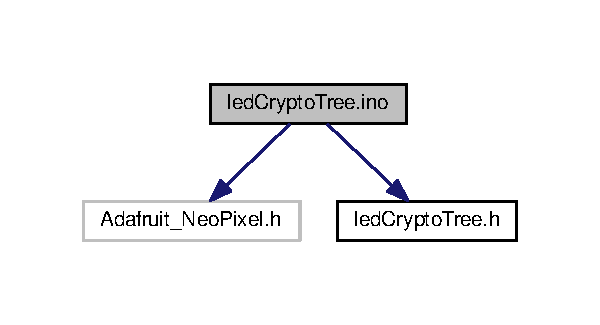
\includegraphics[width=288pt]{ledCryptoTree_8ino__incl}
\end{center}
\end{figure}
\subsection*{Functions}
\begin{DoxyCompactItemize}
\item 
void \hyperlink{ledCryptoTree_8ino_a4fc01d736fe50cf5b977f755b675f11d}{setup} ()
\item 
void \hyperlink{ledCryptoTree_8ino_afe461d27b9c48d5921c00d521181f12f}{loop} ()
\item 
void \hyperlink{ledCryptoTree_8ino_ad4e0c88560cf11558cafaded5334a413}{setup\+Serial} ()
\item 
void \hyperlink{ledCryptoTree_8ino_a3d4a7770febd94a46810f36c3d2ac32e}{setup\+Neopix} ()
\item 
void \hyperlink{ledCryptoTree_8ino_a9e090d395c12709aa3a4ff2754b30828}{parse\+Goals} ()
\item 
void \hyperlink{ledCryptoTree_8ino_a2fb2eb2b13bc6122f9c89d000e2d7d01}{parse\+Serial} ()
\item 
void \hyperlink{ledCryptoTree_8ino_ad5820c78928d904adcd4f284142c506b}{simple\+Fade\+In} (int pin, int speed\+Val)
\item 
void \hyperlink{ledCryptoTree_8ino_a10a605d30a8a525a684e774fba0504d9}{simple\+Fade\+Out} (int pin, int speed\+Val)
\item 
void \hyperlink{ledCryptoTree_8ino_aac3dce34012696fd5c98eb88847e61cd}{color\+Count} (\hyperlink{structLwColor}{Lw\+Color} color, int speed\+Delay, int percent)
\item 
void \hyperlink{ledCryptoTree_8ino_af32fca95526cc1e6753e75cbc621a10a}{cylon\+Bounce} (\hyperlink{structLwColor}{Lw\+Color} color, int eye\+Size, int speed\+Delay, int return\+Delay)
\item 
void \hyperlink{ledCryptoTree_8ino_a96de8ed535af4104229f69adbb6da86c}{color\+Wipe} (\hyperlink{structLwColor}{Lw\+Color} color, int speed\+Delay)
\item 
void \hyperlink{ledCryptoTree_8ino_a68f58d95cb1f5743c670bb22f248fed1}{running\+Lights} (\hyperlink{structLwColor}{Lw\+Color} color, int wave\+Delay)
\item 
void \hyperlink{ledCryptoTree_8ino_ad89dd890beff1d9b79fa3574d096cf7d}{twinkle\+Random} (int count, int speed\+Delay, boolean only\+One)
\item 
void \hyperlink{ledCryptoTree_8ino_ae0c03f03209028b418a16bd771a6f4c0}{snow\+Sparkle} (\hyperlink{structLwColor}{Lw\+Color} color, int sparkle\+Delay, int speed\+Delay)
\item 
void \hyperlink{ledCryptoTree_8ino_a907e4fe4e66cedec66df790c3acbbad7}{sparkle} (\hyperlink{structLwColor}{Lw\+Color} color, int speed\+Delay)
\item 
\hypertarget{ledCryptoTree_8ino_a717066609dbbcc3f6c56fd346e349dae}{void {\bfseries simple\+Wave} (float rate, int cycles, int wait)}\label{ledCryptoTree_8ino_a717066609dbbcc3f6c56fd346e349dae}

\item 
\hypertarget{ledCryptoTree_8ino_ac0a99cebb66e920d0169dda0bbe9d443}{void {\bfseries set\+Pixel} (Neo\+Pix neopix, Pixel pixel, \hyperlink{structLwColor}{Lw\+Color} color)}\label{ledCryptoTree_8ino_ac0a99cebb66e920d0169dda0bbe9d443}

\item 
\hypertarget{ledCryptoTree_8ino_ab9a4798d660acd5ba3a3f47f1f94f7ad}{void {\bfseries set\+Pixel\+Nil} (Neo\+Pix neopix, Pixel pixel)}\label{ledCryptoTree_8ino_ab9a4798d660acd5ba3a3f47f1f94f7ad}

\item 
\hypertarget{ledCryptoTree_8ino_a6eeb037028ab2d28c9357c71c8eae453}{void {\bfseries set\+All} (Neo\+Pix neopix, \hyperlink{structLwColor}{Lw\+Color} color)}\label{ledCryptoTree_8ino_a6eeb037028ab2d28c9357c71c8eae453}

\item 
\hypertarget{ledCryptoTree_8ino_aa71a1cbd34cfb17f4c617214d934ac76}{void {\bfseries set\+All\+Nil} (Neo\+Pix neopix)}\label{ledCryptoTree_8ino_aa71a1cbd34cfb17f4c617214d934ac76}

\item 
\hypertarget{ledCryptoTree_8ino_a383d68f11fa9d78622d5672b343d82cf}{void {\bfseries show} (Neo\+Pix neopix)}\label{ledCryptoTree_8ino_a383d68f11fa9d78622d5672b343d82cf}

\end{DoxyCompactItemize}


\subsection{Function Documentation}
\hypertarget{ledCryptoTree_8ino_aac3dce34012696fd5c98eb88847e61cd}{\index{led\+Crypto\+Tree.\+ino@{led\+Crypto\+Tree.\+ino}!color\+Count@{color\+Count}}
\index{color\+Count@{color\+Count}!led\+Crypto\+Tree.\+ino@{led\+Crypto\+Tree.\+ino}}
\subsubsection[{color\+Count}]{\setlength{\rightskip}{0pt plus 5cm}void color\+Count (
\begin{DoxyParamCaption}
\item[{{\bf Lw\+Color}}]{color, }
\item[{int}]{speed\+Delay, }
\item[{int}]{percent}
\end{DoxyParamCaption}
)}}\label{ledCryptoTree_8ino_aac3dce34012696fd5c98eb88847e61cd}
Counts the color...? Pattern.

A spiral pattern T\+O\+D\+O\+: Get Lindy's interpretation of this pattern.


\begin{DoxyParams}{Parameters}
{\em color} & The color to use (start with?) in \hyperlink{structLwColor}{Lw\+Color} type \\
\hline
{\em speed\+Delay} & The delay used to control the speed (inverse of speed, lower number is faster) \\
\hline
{\em percent} & Percent of...? to...? \\
\hline
\end{DoxyParams}
\hypertarget{ledCryptoTree_8ino_a96de8ed535af4104229f69adbb6da86c}{\index{led\+Crypto\+Tree.\+ino@{led\+Crypto\+Tree.\+ino}!color\+Wipe@{color\+Wipe}}
\index{color\+Wipe@{color\+Wipe}!led\+Crypto\+Tree.\+ino@{led\+Crypto\+Tree.\+ino}}
\subsubsection[{color\+Wipe}]{\setlength{\rightskip}{0pt plus 5cm}void color\+Wipe (
\begin{DoxyParamCaption}
\item[{{\bf Lw\+Color}}]{color, }
\item[{int}]{speed\+Delay}
\end{DoxyParamCaption}
)}}\label{ledCryptoTree_8ino_a96de8ed535af4104229f69adbb6da86c}
Pattern that wipes with color.

A vertical Pattern T\+O\+D\+O\+: Get Lindy's interpretation of this pattern.


\begin{DoxyParams}{Parameters}
{\em color} & The color to use (start with?) in \hyperlink{structLwColor}{Lw\+Color} type \\
\hline
{\em speed\+Delay} & The delay used to control the speed (inverse of speed, lower number is faster) \\
\hline
\end{DoxyParams}
\hypertarget{ledCryptoTree_8ino_af32fca95526cc1e6753e75cbc621a10a}{\index{led\+Crypto\+Tree.\+ino@{led\+Crypto\+Tree.\+ino}!cylon\+Bounce@{cylon\+Bounce}}
\index{cylon\+Bounce@{cylon\+Bounce}!led\+Crypto\+Tree.\+ino@{led\+Crypto\+Tree.\+ino}}
\subsubsection[{cylon\+Bounce}]{\setlength{\rightskip}{0pt plus 5cm}void cylon\+Bounce (
\begin{DoxyParamCaption}
\item[{{\bf Lw\+Color}}]{color, }
\item[{int}]{eye\+Size, }
\item[{int}]{speed\+Delay, }
\item[{int}]{return\+Delay}
\end{DoxyParamCaption}
)}}\label{ledCryptoTree_8ino_af32fca95526cc1e6753e75cbc621a10a}
Pattern that bounds back and forth like a clasic cylon's eyes.

A spiral pattern T\+O\+D\+O\+: Get Lindy's full interpretation of this pattern.


\begin{DoxyParams}{Parameters}
{\em color} & The color to use (start with?) in \hyperlink{structLwColor}{Lw\+Color} type \\
\hline
{\em eye\+Size} & The size of the... Eyes? \\
\hline
{\em speed\+Delay} & The delay used to control the speed (inverse of speed, lower number is faster) \\
\hline
{\em return\+Delay} & Rebounding delay? \\
\hline
\end{DoxyParams}
\hypertarget{ledCryptoTree_8ino_afe461d27b9c48d5921c00d521181f12f}{\index{led\+Crypto\+Tree.\+ino@{led\+Crypto\+Tree.\+ino}!loop@{loop}}
\index{loop@{loop}!led\+Crypto\+Tree.\+ino@{led\+Crypto\+Tree.\+ino}}
\subsubsection[{loop}]{\setlength{\rightskip}{0pt plus 5cm}void loop (
\begin{DoxyParamCaption}
{}
\end{DoxyParamCaption}
)}}\label{ledCryptoTree_8ino_afe461d27b9c48d5921c00d521181f12f}
m\+Controller loop function (control loop) \hypertarget{ledCryptoTree_8ino_a9e090d395c12709aa3a4ff2754b30828}{\index{led\+Crypto\+Tree.\+ino@{led\+Crypto\+Tree.\+ino}!parse\+Goals@{parse\+Goals}}
\index{parse\+Goals@{parse\+Goals}!led\+Crypto\+Tree.\+ino@{led\+Crypto\+Tree.\+ino}}
\subsubsection[{parse\+Goals}]{\setlength{\rightskip}{0pt plus 5cm}void parse\+Goals (
\begin{DoxyParamCaption}
{}
\end{DoxyParamCaption}
)}}\label{ledCryptoTree_8ino_a9e090d395c12709aa3a4ff2754b30828}
Parse the current goal in to patterns

\begin{DoxySeeAlso}{See also}
enum \hyperlink{ledCryptoTree_8h_a0ba78d87f754b7f0ab05e1534dfb54f4}{Goals} 
\end{DoxySeeAlso}
\hypertarget{ledCryptoTree_8ino_a2fb2eb2b13bc6122f9c89d000e2d7d01}{\index{led\+Crypto\+Tree.\+ino@{led\+Crypto\+Tree.\+ino}!parse\+Serial@{parse\+Serial}}
\index{parse\+Serial@{parse\+Serial}!led\+Crypto\+Tree.\+ino@{led\+Crypto\+Tree.\+ino}}
\subsubsection[{parse\+Serial}]{\setlength{\rightskip}{0pt plus 5cm}void parse\+Serial (
\begin{DoxyParamCaption}
{}
\end{DoxyParamCaption}
)}}\label{ledCryptoTree_8ino_a2fb2eb2b13bc6122f9c89d000e2d7d01}
Parse the incoming serial data to set Goal progression and/or patterns

\begin{DoxySeeAlso}{See also}
Goal 
\end{DoxySeeAlso}
\hypertarget{ledCryptoTree_8ino_a68f58d95cb1f5743c670bb22f248fed1}{\index{led\+Crypto\+Tree.\+ino@{led\+Crypto\+Tree.\+ino}!running\+Lights@{running\+Lights}}
\index{running\+Lights@{running\+Lights}!led\+Crypto\+Tree.\+ino@{led\+Crypto\+Tree.\+ino}}
\subsubsection[{running\+Lights}]{\setlength{\rightskip}{0pt plus 5cm}void running\+Lights (
\begin{DoxyParamCaption}
\item[{{\bf Lw\+Color}}]{color, }
\item[{int}]{wave\+Delay}
\end{DoxyParamCaption}
)}}\label{ledCryptoTree_8ino_a68f58d95cb1f5743c670bb22f248fed1}
Pattern that runs down the string with color.

A vertical Pattern T\+O\+D\+O\+: Get Lindy's interpretation of this pattern.


\begin{DoxyParams}{Parameters}
{\em color} & The color to use (start with?) in \hyperlink{structLwColor}{Lw\+Color} type \\
\hline
{\em wave\+Delay} & The delay used to control the speed (inverse of speed, lower number is faster) \\
\hline
\end{DoxyParams}
\hypertarget{ledCryptoTree_8ino_a4fc01d736fe50cf5b977f755b675f11d}{\index{led\+Crypto\+Tree.\+ino@{led\+Crypto\+Tree.\+ino}!setup@{setup}}
\index{setup@{setup}!led\+Crypto\+Tree.\+ino@{led\+Crypto\+Tree.\+ino}}
\subsubsection[{setup}]{\setlength{\rightskip}{0pt plus 5cm}void setup (
\begin{DoxyParamCaption}
{}
\end{DoxyParamCaption}
)}}\label{ledCryptoTree_8ino_a4fc01d736fe50cf5b977f755b675f11d}
m\+Controller setup function (initilizer) \hypertarget{ledCryptoTree_8ino_a3d4a7770febd94a46810f36c3d2ac32e}{\index{led\+Crypto\+Tree.\+ino@{led\+Crypto\+Tree.\+ino}!setup\+Neopix@{setup\+Neopix}}
\index{setup\+Neopix@{setup\+Neopix}!led\+Crypto\+Tree.\+ino@{led\+Crypto\+Tree.\+ino}}
\subsubsection[{setup\+Neopix}]{\setlength{\rightskip}{0pt plus 5cm}void setup\+Neopix (
\begin{DoxyParamCaption}
{}
\end{DoxyParamCaption}
)}}\label{ledCryptoTree_8ino_a3d4a7770febd94a46810f36c3d2ac32e}
Setup for Neopixel objects \hypertarget{ledCryptoTree_8ino_ad4e0c88560cf11558cafaded5334a413}{\index{led\+Crypto\+Tree.\+ino@{led\+Crypto\+Tree.\+ino}!setup\+Serial@{setup\+Serial}}
\index{setup\+Serial@{setup\+Serial}!led\+Crypto\+Tree.\+ino@{led\+Crypto\+Tree.\+ino}}
\subsubsection[{setup\+Serial}]{\setlength{\rightskip}{0pt plus 5cm}void setup\+Serial (
\begin{DoxyParamCaption}
{}
\end{DoxyParamCaption}
)}}\label{ledCryptoTree_8ino_ad4e0c88560cf11558cafaded5334a413}
Setup for serial connection \hypertarget{ledCryptoTree_8ino_ad5820c78928d904adcd4f284142c506b}{\index{led\+Crypto\+Tree.\+ino@{led\+Crypto\+Tree.\+ino}!simple\+Fade\+In@{simple\+Fade\+In}}
\index{simple\+Fade\+In@{simple\+Fade\+In}!led\+Crypto\+Tree.\+ino@{led\+Crypto\+Tree.\+ino}}
\subsubsection[{simple\+Fade\+In}]{\setlength{\rightskip}{0pt plus 5cm}void simple\+Fade\+In (
\begin{DoxyParamCaption}
\item[{int}]{pin, }
\item[{int}]{speed\+Val}
\end{DoxyParamCaption}
)}}\label{ledCryptoTree_8ino_ad5820c78928d904adcd4f284142c506b}
Simple fade-\/in pattern for non-\/addressable lights.

A simple pattern Controls a single analog pin.


\begin{DoxyParams}{Parameters}
{\em pin} & The pin to control \\
\hline
{\em speed\+Val} & The delay used to control the speed (inverse of speed, lower number is faster) \\
\hline
\end{DoxyParams}
\hypertarget{ledCryptoTree_8ino_a10a605d30a8a525a684e774fba0504d9}{\index{led\+Crypto\+Tree.\+ino@{led\+Crypto\+Tree.\+ino}!simple\+Fade\+Out@{simple\+Fade\+Out}}
\index{simple\+Fade\+Out@{simple\+Fade\+Out}!led\+Crypto\+Tree.\+ino@{led\+Crypto\+Tree.\+ino}}
\subsubsection[{simple\+Fade\+Out}]{\setlength{\rightskip}{0pt plus 5cm}void simple\+Fade\+Out (
\begin{DoxyParamCaption}
\item[{int}]{pin, }
\item[{int}]{speed\+Val}
\end{DoxyParamCaption}
)}}\label{ledCryptoTree_8ino_a10a605d30a8a525a684e774fba0504d9}
Simple fade-\/out pattern for non-\/addressable lights.

A simple pattern Controls a single analog pin.


\begin{DoxyParams}{Parameters}
{\em pin} & The pin to control \\
\hline
{\em speed\+Val} & The delay used to control the speed (inverse of speed, lower number is faster) \\
\hline
\end{DoxyParams}
\hypertarget{ledCryptoTree_8ino_ae0c03f03209028b418a16bd771a6f4c0}{\index{led\+Crypto\+Tree.\+ino@{led\+Crypto\+Tree.\+ino}!snow\+Sparkle@{snow\+Sparkle}}
\index{snow\+Sparkle@{snow\+Sparkle}!led\+Crypto\+Tree.\+ino@{led\+Crypto\+Tree.\+ino}}
\subsubsection[{snow\+Sparkle}]{\setlength{\rightskip}{0pt plus 5cm}void snow\+Sparkle (
\begin{DoxyParamCaption}
\item[{{\bf Lw\+Color}}]{color, }
\item[{int}]{sparkle\+Delay, }
\item[{int}]{speed\+Delay}
\end{DoxyParamCaption}
)}}\label{ledCryptoTree_8ino_ae0c03f03209028b418a16bd771a6f4c0}
Pattern that sparkles like snow!

A vertical pattern

\+: Get Lindy's interpretation of this pattern.


\begin{DoxyParams}{Parameters}
{\em color} & The color to use (start with?) in \hyperlink{structLwColor}{Lw\+Color} type \\
\hline
{\em sparkle\+Delay} & The delay used to control the duration of a \char`\"{}sparkle\char`\"{}? \\
\hline
{\em speed\+Delay} & The delay used to control the speed (inverse of speed, lower number is faster) \\
\hline
\end{DoxyParams}
\hypertarget{ledCryptoTree_8ino_a907e4fe4e66cedec66df790c3acbbad7}{\index{led\+Crypto\+Tree.\+ino@{led\+Crypto\+Tree.\+ino}!sparkle@{sparkle}}
\index{sparkle@{sparkle}!led\+Crypto\+Tree.\+ino@{led\+Crypto\+Tree.\+ino}}
\subsubsection[{sparkle}]{\setlength{\rightskip}{0pt plus 5cm}void sparkle (
\begin{DoxyParamCaption}
\item[{{\bf Lw\+Color}}]{color, }
\item[{int}]{speed\+Delay}
\end{DoxyParamCaption}
)}}\label{ledCryptoTree_8ino_a907e4fe4e66cedec66df790c3acbbad7}
Pattern that sparkles.

A vertical pattern

\+: Jane, you left off here 'cause brain tired. \+: Get Lindy's interpretation of this pattern.


\begin{DoxyParams}{Parameters}
{\em color} & The color to use (start with?) in \hyperlink{structLwColor}{Lw\+Color} type \\
\hline
{\em sparkle\+Delay} & The delay used to control the duration of a \char`\"{}sparkle\char`\"{}? \\
\hline
{\em speed\+Delay} & The delay used to control the speed (inverse of speed, lower number is faster) \\
\hline
\end{DoxyParams}
\hypertarget{ledCryptoTree_8ino_ad89dd890beff1d9b79fa3574d096cf7d}{\index{led\+Crypto\+Tree.\+ino@{led\+Crypto\+Tree.\+ino}!twinkle\+Random@{twinkle\+Random}}
\index{twinkle\+Random@{twinkle\+Random}!led\+Crypto\+Tree.\+ino@{led\+Crypto\+Tree.\+ino}}
\subsubsection[{twinkle\+Random}]{\setlength{\rightskip}{0pt plus 5cm}void twinkle\+Random (
\begin{DoxyParamCaption}
\item[{int}]{count, }
\item[{int}]{speed\+Delay, }
\item[{boolean}]{only\+One}
\end{DoxyParamCaption}
)}}\label{ledCryptoTree_8ino_ad89dd890beff1d9b79fa3574d096cf7d}
Pattern that randomly \char`\"{}twinkles\char`\"{} lights in the string.

A vertical pattern

\+: Get Lindy's interpretation of this pattern.


\begin{DoxyParams}{Parameters}
{\em count} & The number of lights to twinkle in the string (Sets up density) \\
\hline
{\em speed\+Delay} & The delay used to control the speed (inverse of speed, lower number is faster) \\
\hline
{\em only\+One} & Only twinkles one light at a time? \\
\hline
\end{DoxyParams}

%--- End generated contents ---

% Index
\newpage
\phantomsection
\addcontentsline{toc}{chapter}{Index}
\printindex

\end{document}
